% ######################################################################################################################
%         Visualization
% ######################################################################################################################

\chapter{Visualization}
\label{ch:Visualization}

\paperbox{
    This chapter is based on parts of the peer-reviewed publication:
}{\paperpppp}{
    \textbf{Contributions:} Lucas Czech... Alexandros Stamatakis...
}

% ######################################################################################################################
%         Background and Motivation
% ######################################################################################################################

\section{Background and Motivation}
\label{ch:Visualization:sec:Motivation}

When analyzing a set of metagenomic sequence samples (\secref{ch:Foundations:sec:SequenceAnalysis:sub:Metagenomics})
using phylogenetic placement (\secref{ch:Foundations:sec:PhylogeneticPlacement}),
a first step is often to visualize the data.
% A first step in analyzing phylogenetic placement data is often to visualize them.
For small samples, it is possible to mark individual placement locations on the \acf{RT},
as offered for example by \toolname{iTOL} \cite{Letunic2016},
or even to create a tree where the most probable placement per \acf{QS} is attached as a new branch,
as implemented in the \toolname{guppy} tool from the \toolname{pplacer} suite \cite{Matsen2010},
\toolname{RAxML-EPA} \cite{Berger2011,Stamatakis2014}, and our tool \toolname{gappa}.
\todo{link to supplement or paper, or something}
For larger samples, one can alternatively display the per-edge placement mass,
either by adjusting the line widths of the edges according to their mass, or by using a color scale,
as offered in \toolname{ggtree} \cite{Yu2017}, \toolname{guppy}, and \toolname{gappa}.
Using per-edge colors corresponds to binning all placements of an edge into one bin
(see \secref{ch:Foundations:sec:PhylogeneticPlacement:sub:PlacementProcessing:par:EdgeMasses}).
%it is thinkable to use multiple bins instead, too, resulting in edges split into segments with different colors.
For large datasets, the per-edge masses can vary by several orders of magnitude.
In such cases, it is often preferable to use a logarithmic scaling, as shown in \citeay{Mahe2017}.
In addition to visualizing each sample separately, the average mass distribution
(after \emph{squashing} the masses,
see \secref{ch:Foundations:sec:PhylogeneticPlacement:sub:PlacementProcessing:par:EdgeMasses})
% provides an overview of a set of samples.
visually summarizes a set of samples.

The visualizations provide an overview of the species abundances over the tree.
They can be regarded as a more detailed version of abundance charts \cite{Huttenhower2012},
which are typically shown in the form of pie or bar plots \cite{Faust2015,Mahe2017,Lentendu2018}.
For instance, \figref{fig:abundances_comparison} shows a comparison of a simple abundances pie chart
compared to a visualization of per-branch abundances on a reference tree for the same dataset.
Although there exist more advanced variants such as
hierarchical pie charts, for instance as offered by the \toolname{Krona} tool \cite{Ondov2011},
it should be apparent that the tree visualization provides more detailed information.
In \figref{fig:abundances_comparison:sub:branch_colors}, we combined the information of the pie chart
with the tree visualization by displaying the abundances next to each clade.
% Those two figures can even be combined into one by adding brackets with abundances
% around the clades of the tree when drawing it.
% When drawing the tree, abundances can also be annotated around its clades,
% effectively combining those two figures into one.

\begin{figure}[!ht]
    \centering
    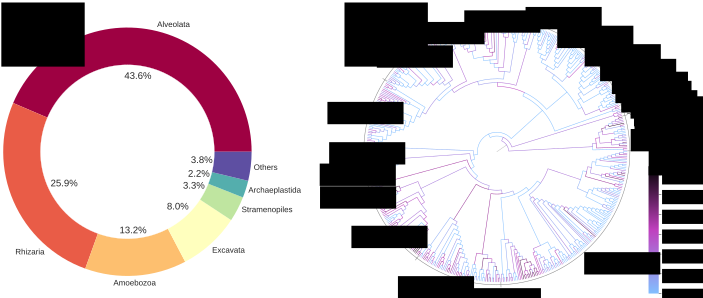
\includegraphics[width=\linewidth]{abundances_comparison.pdf}
    \begin{subfigure}{0pt}
        \phantomcaption
        \label{fig:abundances_comparison:sub:pie_chart}
    \end{subfigure}
    \begin{subfigure}{0pt}
        \phantomcaption
        \label{fig:abundances_comparison:sub:branch_colors}
    \end{subfigure}
    \caption[Visualizations of sequence abundances]{
        \textbf{Visualizations of sequence abundances.}
        The figure shows an example of
        \subref{fig:abundances_comparison:sub:pie_chart} a typical pie chart of taxonomic abundances and
        \subref{fig:abundances_comparison:sub:branch_colors} the substantially more informative
        per-branch mass visualization using phylogenetic placement on a reference tree.
        The data is from \citeay{Mahe2017}, see \appref{supp:sec:DetailsEmpiricalDatasets:sub:NTS} for details.
%         Note that pie charts are usually not considered good visualization practice,
%         and thus better use bar plots. but, it seems to be a default in many papers...
%         \\
        The branches of the tree are colored by abundances on a logarithmic scale,
        and clades of the tree are annotated with the per-clade abundances,
        effectively combining the information of the pie chart with the tree visualization.
    }
    \label{fig:abundances_comparison}
\end{figure}

% A more detailed visualization can be obtained by showing the abundances per taxon and per sample.
% which is often used for OTU trees, where a heat map can show the abundances of the OTUS at the tips of the tree.
A more detailed visualization of the abundances per taxon and per sample 
can be obtained via a heat map that shows the per-sample abundances at the tips of the tree.
This is often used for OTU trees, where tips correspond to the OTUs that the tree was inferred from.
This can be extended to placements by also showing abundances/masses at the inner edges, 
as shown in \figref{fig:heat_tree}.
The figure shows the placements per edge and per sample for the \ac{BV} dataset;
see \secref{supp:sec:DetailsEmpiricalDatasets:sub:BV} for details on this dataset.

% for instance in form of a heat map as exemplified in \figref{fig:heat_tree}.
% Typically, these visualizations are used for trees inferred from OTU sequences,
% meaning that abundances 
% typically, for otus abundances at tips.
% can however be extended to placements by also showing masses at inner branches,

\begin{figure}[!htbp]
    \centering
    \vspace{-1em}
    \includegraphics[width=\linewidth]{heat_tree.pdf}
    \caption[Visualization of per-edge and per-sample masses of the BV dataset]{
        \textbf{Visualization of per-edge and per-sample masses of the BV dataset.}
        The figure provides an overview of the placement of the \ac{BV} dataset:
        The left hand side shows a condensed version of the original reference tree of \citeay{Srinivasan2012},
        colored by log-scaled placement mass of all samples accumulated.
        For clarity and simplicity, in this figure we used a reference tree
        built from the consensus sequences of each original reference taxon,
        so that each species is represented by exactly one tip here.
        The \taxonname{Lactobacillus} clade is highlighted in the tree, which is an important clade for this dataset.
        \\
        The right hand side shows a heat map that further resolves the placement masses per sample:
        Each row corresponds to a branch of the tree on the left (note that dashed lines also start from inner branches),
        and each column represents one sample.
        The values are log-centered in order to
        be consistent with typical OTU abundance heat map representations \cite{Washburne2017a}.
%         for example as in \citeay{Washburne2017a}.
        The samples/columns are sorted by their Nugent score,
        from \num{0} at the left for the healthy patients to \num{10} at the right for the sick ones.
        The Nugent score of each sample is also shown at the top as a blue to red bar.
        % ranging from 0 (healthy) to 10 (severe illness).
    }
    \label{fig:heat_tree}
\end{figure}

On the left hand side of \figref{fig:heat_tree}, note the two particularly dark branches, 
\taxonname{Lactobacillus iners} and \taxonname{Lactobacillus crispatus},
which are the major species associated with a healthy vaginal microbiome \cite{Srinivasan2012}.
This can also be seen on the right hand side of the figure,
where the high abundance of \taxonname{Lactobacillus} in healthy patients
is visible in the lower part of the matrix,
while the diseased patients exhibit high placement masses at several other taxa \cite{Srinivasan2012}.

Such visualizations directly depict the placement masses on the tree.
When visualizing the accumulated masses of multiple samples at once,
it is important to chose an appropriate normalization strategy for the task at hand,
as explained in \secref{ch:Foundations:sec:PhylogeneticPlacement:sub:PlacementProcessing}.
For example, if samples represent different locations, one might prefer to use normalized masses,
as comparing relative abundances is common for this type of data.
On the other hand, if samples from the same location are combined
(e.g., from different points in time, or different size fractions),
it might be preferable to use absolute abundances instead,
so that the total number of sequences per sample can be visualized.

When placing OTUs (see \secref{ch:Foundations:sec:PhylogeneticPlacement:sub:PlacementProcessing}),
or ignoring sequence abundances, the resulting visualizations can be interpreted as a depiction of species diversity.
Moreover, these visualizations can be used to assess the quality of the \ac{RT}.
% No ``zone'' here? Micah will be disappointed...
% The inner edges of the \ac{RT} form a zone of older evolutionary relationships.
% Placements into that zone may indicate that appropriate reference sequences
For example, placements into inner branches of the \ac{RT} may indicate that appropriate reference sequences
(i) have either not been included or (ii) are simply not available yet.
This complements the sequence filtering that relies on so-called backbone trees
as previously described in \secref{ch:AutomaticTrees:sec:Methods:sub:MultilevelPlacement}.

These visualizations are useful tools for initial dataset and feature exploration in terms of species abundances.
However, when working with multiple samples,
they do not immediately reveal relative differences between samples
that might hint at underlying biological or ecological properties of the samples or their environment.
% Edge PCA \cite{Matsen2011a} (see \secref{ch:Foundations:sec:PhylogeneticPlacement:sub:ExistingMethods:par:EdgePCA})
% is a method for such types of analyses,
% which however yields plots that are...

% ######################################################################################################################
%         Methods and Implementation
% ######################################################################################################################

\section{Methods and Implementation}
\label{ch:Visualization:sec:Methods}

Here, we introduce visualization methods for phylogenetic placement of a set of metagenomic sequence samples
that highlight (1) regions of the tree with a high variance in their placement distribution (called \emph{Edge Dispersion}),
and (2) regions with a high correlation to meta-data features (called \emph{Edge Correlation}).

Both methods take as input a set of samples, each consisting of a set of \acf{QS} placed on a fixed \acf{RT}.
They then use the edge masses matrix and the edge imbalances matrix
as introduced in \secref{ch:Foundations:sec:PhylogeneticPlacement:sub:PlacementProcessing}
to calculate per-branch quantities, which are subsequently visualized on the \ac{RT}.

% ======================================================================================================================
%         Edge Dispersion
% ======================================================================================================================

\subsection{Edge Dispersion}
\label{ch:Visualization:sec:Methods:sub:EdgeDispersion}

The Edge Dispersion is derived from the edge masses or edge imbalances matrix
(\secref{ch:Foundations:sec:PhylogeneticPlacement:sub:PlacementProcessing})
% as introduced in \secref{ch:Foundations:sec:PhylogeneticPlacement:sub:PlacementProcessing}
by calculating a measure of dispersion for each matrix column, for example, the standard deviation $\sigma$.
Because each column corresponds to an edge, this information can be mapped back to the tree,
and visualized, for instance, via color coding.
% Edges with a high variance indicate parts of the tree with...
This allows to examine which edges exhibit a high heterogeneity of placement masses across samples,
% vary in terms of their placements,
and hence indicates which edges discriminate samples.

As the abundances of different species, and hence also the edge mass values, can span many orders of magnitude,
% As edge mass values can span many orders of magnitude,
it might be necessary to scale the variance logarithmically. %, % as shown in \figref{fig:var_cor:sub:em_varl},
%or to use some other form of normalization.
Often, one is more interested in the branches with high placement mass,
as they comprise the most abundant species in the samples.
In these cases, using the standard deviation or variance is appropriate,
as they also indicate the mean per-edge mass.
On the other hand, by calculating the per-edge Index of Dispersion \cite{Everitt2010},
that is, the variance-mean-ratio $\sfrac{\sigma^2}{\mu}$,
differences on edges with little mass also become visible.
Note that this is a valid operation, as edge masses are non-negative count variables.
The Index of Dispersion is useful to explore heterogeneity on edges with low species abundances.
% \todo{furthermore, Index of Dispersion is often used to compare to a Poisson distribution,
% which we however do not expect from masses. maybe this is still interesting}

As Edge Dispersion relates placement masses from different samples to each other,
the choice of the normalization strategy {\em is} important
(see also \secref{ch:Foundations:sec:PhylogeneticPlacement:sub:PlacementProcessing}).
When using normalized masses, the magnitude of dispersion values needs to be cautiously interpreted \cite{Lovell2015}.
The Edge Dispersion can also be calculated for edge imbalances in form of the standard deviation.
As edge imbalances are usually normalized to $[ -1.0, 1.0 ]$,
their dispersion can be visualized directly without any further normalization steps.
However, because imbalances can be negative, the Index of Dispersion is not applicable to them.
An example for an Edge Dispersion visualization is shown in \figref{fig:var_cor:sub:em_varl},
and discussed in \secref{ch:Visualization:sec:Results}.

\begin{figure}[!ht]
    \centering
    \includegraphics[width=\linewidth]{var_cor.pdf}
    \begin{subfigure}{0pt}
        \phantomcaption
        \label{fig:var_cor:sub:em_varl}
    \end{subfigure}
    \begin{subfigure}{0pt}
        \phantomcaption
        \label{fig:var_cor:sub:ei_var}
    \end{subfigure}
    \caption[Examples of Edge Dispersion and Edge Correlation]{
        \textbf{Examples of Edge Dispersion and Edge Correlation.}
        We applied our novel visualization methods to the \acf{BV} dataset
        (see \appref{supp:sec:DetailsEmpiricalDatasets:sub:BV} for details)
        to compare them to the existing data analysis methods.
%         See \cite{Srinivasan2012} for details of the dataset and its interpretation.
        \subref{fig:var_cor:sub:em_varl}
        Edge Dispersion, measured as the standard deviation of the edge masses across samples, logarithmically scaled.
        \subref{fig:var_cor:sub:ei_var}
        Edge Correlation, in form of Spearman's Rank Correlation Coefficient
        between the edge imbalances and the Nugent score.
        Tip edges are gray, because they do not have a meaningful imbalance.
        This example also shows the characteristics of edge masses and edge imbalances:
        The former highlights individual edges, the latter highlights paths to clades.
%         Note that in this case, both methods highlight similar parts of the tree.
    }
    \label{fig:var_cor}
\end{figure}

% ======================================================================================================================
%         Edge Correlation
% ======================================================================================================================

\subsection{Edge Correlation}
\label{ch:Visualization:sec:Methods:sub:EdgeCorrelation}

In addition to the per-edge masses, the Edge Correlation can further
take a specific meta-data feature into account, that is, a column of the meta-data matrix.
The Edge Correlation is calculated as the correlation between each edge column and the feature column,
for example by using the Pearson Correlation Coefficient or Spearman's Rank Correlation Coefficient \cite{Everitt2010}.
This yields a per-edge correlation of the placement masses or imbalances with the specific meta-data feature,
and can again be visualized by color coding the edges.


% The \bar command is too short for $m$. Use a better one - which however is too short again for $c$...
% So, let's use each of them where appropriate. Not satisfying, but does the job.
% https://tex.stackexchange.com/a/22134/171851
% \newcommand{\overbar}[1]{\mkern 1.5mu\overline{\mkern-1.5mu#1\mkern-1.5mu}\mkern 1.5mu}
\newcommand{\barredc}{\mkern 1mu\overline{\mkern-1mu{}c\mkern1mu}\mkern-1mu\;\!}
\newcommand{\barredm}{\mkern 1.5mu\overline{\mkern-1.5mu{}m\mkern-1.5mu}\mkern 1.5mu}

The Pearson Correlation Coefficient $r$ between the per-edge mass or imbalance column $c$ (with average $\barredc$)
and the meta-data column $m$ (with average $\barredm$) for a set of $s$ samples is calculated as

\begin{equation}
    \label{ch:Visualization:eq:PCC}
    r ~=~ \frac{ \sum_{i=1}^{s} (c_i - \barredc)(m_i - \barredm) }{ \sqrt{ \sum_{i=1}^{s} (c_i - \barredc)^2 } ~ \sqrt{ \sum_{i=1}^{s} (m_i - \barredm)^2 } }
%     r =\frac{\sum ^n _{i=1}(x_i - \bar{x})(y_i - \bar{y})}{\sqrt{\sum ^n _{i=1}(x_i - \bar{x})^2} \sqrt{\sum ^n _{i=1}(y_i - \bar{y})^2}}
\end{equation}

Spearman's Rank Correlation Coefficient is calculated in the same way, but instead of using the actual values
of the matrix columns, their ranking numbers are used.
That is, the values are reduced to ordinal numbers, where the lowest value is transformed into \num{1},
the second lowest value into \num{2}, etc.
As a consequence, instead of a linear correlation, this coefficient calculates the strength of monotonic correlations.

Both variants are inexpensive to calculate and hence scale well to large datasets.
As typical correlation coefficients are within $[ -1.0, 1.0 \,]$, there is again no need for further normalization.
This yields a tree where edges or clades with either a high linear or high monotonic correlation
with the selected meta-data feature are highlighted.
\figref{fig:var_cor:sub:ei_var} shows an exemplary visualization of this method.

In contrast to Edge PCA \cite{Matsen2011a} that can use meta-data features to annotate samples in its scatter plots
(see \secref{ch:Foundations:sec:PhylogeneticPlacement:sub:ExistingMethods:par:EdgePCA}),
our Edge Correlation method directly displays the influence of a feature on the branches or clades of the tree.
It can thus, for example, help to identify and visualize dependencies
between species abundances and environmental factors such as temperature or nutrient levels.
Again, the choice of the normalization strategy is important to draw meaningful conclusions.
However, the correlation is \emph{not} calculated between samples or sequence abundances.
% the masses are not put into correlation with each other
Hence, even when using normalized samples, %that is, working with compositional data,
the pitfalls induced by correlations of compositional data \cite{Lovell2015} do not apply here.

% The method further bears some conceptual similarity to methods
% such as Phylo\-Factor \cite{Washburne2017a} and Balance Trees \cite{Morton2017},
% which we briefly described in \secref{ch:Foundations:sec:PhylogeneticPlacement:sub:PlacementProcessing:par:EdgeImbalances}.
% These methods are also able to take meta-data features into account and
% can hence identify relationships between changes in environmental variables and changes in the per-node balance.
% They differ from our Edge Correlation as described before:
% Balances are a property of nodes, not edges, and they do not use a fixed reference tree.
% We outline a potential transfer of the Edge Correlation concept to balances in \chpref{ch:ConclusionOutlook:par:AnalysisMethods}.

The method further bears some conceptual similarity to Phylofactorization \cite{Washburne2017a},
for which we present adaptation to phylogenetic placements in \chpref{ch:Factorization}.
Phylofactorization also takes meta-data features into account and can hence identify relationships
between changes in environmental variables and changes in abundances in clades of the tree.
It typically uses linear regression in form of a \acf{GLM} to assess these relationships.
Note that the correlation coefficient used in our Edge Correlation
can be interpreted as the slope of the regression line of the standardized values,
which establishes a connection between Edge Correlation and Phylofactorization.
The advantage of using correlations here instead of a \ac{GLM} lies in its simplicity for the interpretation of results:
% While regression can take multiple meta-data features into account at the same it,
We are here interested in whether changes in a meta-data feature
lead to an increase or decrease of abundances on branches or in clades of the tree.
Using a \ac{GLM} for this purpose would not yield any advantage.

% ######################################################################################################################
%         Evaluation and Results
% ######################################################################################################################

\section{Evaluation and Results}
\label{ch:Visualization:sec:Results}

% ----------------------------------------------------------------------------------------------------------------------
%     BV Dataset
% ----------------------------------------------------------------------------------------------------------------------

\subsection{BV Dataset}
\label{ch:Visualization:sec:Results:sub:BVDataset}

We re-analyzed the \acf{BV} dataset (see \appref{supp:sec:DetailsEmpiricalDatasets:sub:BV} for details)
by inferring a tree from the original reference sequence set
and conducting phylogenetic placement of the \num{220} samples.
The characteristics of this dataset were already explored by \citeay{Srinivasan2012} and \citeay{Matsen2011a}.
We use it here to give exemplary interpretations of our Edge Dispersion and Edge Correlation methods,
and to evaluate them in comparison to existing methods.

\figref{fig:var_cor} shows our novel visualizations of the \ac{BV} dataset.
Edge Dispersion is shown in \figref{fig:var_cor:sub:em_varl},
% using the standard deviation of the edge masses, logarithmically scaled.
while \figref{fig:var_cor:sub:ei_var} shows the Edge Correlation with the Nugent score. % with the edge imbalances.
The Nugent score \cite{Nugent1991} is a clinical standard for the diagnosis of Bacterial Vaginosis,
ranging from \num{0} (healthy) to \num{10} (severe illness).
Bacterial Vaginosis (BV) is a disease of the vagina
that manifests itself in form of an abnormal vaginal microbiome \cite{Srinivasan2012}.

The connection between the Nugent score and the abundance of placements on particular edges
was already explored by \citeay{Matsen2011a}, but only visualized indirectly (i.e., not on the \ac{RT} itself).
For example, Figure~6 of the original study \cite{Matsen2011a}
plots the first two Edge PCA components colorized by the Nugent score.
We recalculated this figure for comparison, and show it later in \figref{fig:kmeans_all:sub:epca_ns}.

In contrast to this, our Edge Correlation measure directly reveals
the connection between the Nugent score and placements on the reference tree:
The clade on the left hand side of the tree, to which the red and orange branches lead,
are \taxonname{Lactobacillus iners} and \taxonname{Lactobacillus crispatus}, respectively,
which were identified in \citeay{Srinivasan2012} to be associated with a healthy vaginal microbiome.
Thus, their presence in a sample is anti-correlated with the Nugent score, which is lower for healthy individuals.
The branches leading to this clade are therefore colored in red.
On the other hand, there are several other clades that exhibit a positive correlation with the Nugent score,
that is, were green and blue paths lead to in the figure,
again a finding already reported in \citeay{Srinivasan2012}.

Both trees in \figref{fig:var_cor} highlight the same parts of the tree:
The dark branches with high deviation in \figref{fig:var_cor:sub:em_varl} represent clades
attached to either highly correlated (blue) or anti-correlated (red) paths \figref{fig:var_cor:sub:ei_var}.
This indicates that edges that have a high dispersion
also exhibit variation in placement mass between samples of different Nugent score.
This indicates that both methods reveal the clades that are relevant for discriminating among the samples of this dataset.

We further compared our methods to the visualization of Edge PCA components on the reference tree.
To this end, we recalculated Figures~4 and 5 of \citeay{Matsen2011a},
and visualized them with our color scheme in \figref{fig:epca} for ease of comparison.
The figures show the first two components of Edge PCA, mapped back to the branches of the \ac{RT}.
The first component, \figref{fig:epca:sub:comp1},
reveals that the \taxonname{Lactobacillus} clade represents the axis with the highest heterogeneity across samples,
while the second component, \figref{fig:epca:sub:comp2},
further distinguishes between the two aforementioned clades within the \taxonname{Lactobacilli}.
As shown in \figref{fig:var_cor:sub:ei_var}, Edge Correlation also highlights the \taxonname{Lactobacillus} clade,
but does not distinguish further between its sub-clades.
This is because a high Nugent score is associated
with a high abundance of placements in either of the two relevant \taxonname{Lactobacillus} clades.
% In other words, Edge Correlation only reveals information that is associated with the used meta-data feature.

% -----------------------------------------
%     Edge PCA
% -----------------------------------------

\begin{figure}[hpbt]
    \centering
    \vspace*{1em}
    \includegraphics[width=\linewidth]{epca.pdf}
    \vspace*{-1em}
    \begin{subfigure}{0pt}
        \phantomcaption
        \label{fig:epca:sub:comp1}
    \end{subfigure}
    \begin{subfigure}{0pt}
        \phantomcaption
        \label{fig:epca:sub:comp2}
    \end{subfigure}
    \caption[Recalculation of the Edge PCA tree visualization]{
        \textbf{Recalculation of the Edge PCA tree visualization.}
        Subfigures~\subref{fig:epca:sub:comp1} and \subref{fig:epca:sub:comp2} are recalculations
        of Figures 4 and 5 of \citeay{Matsen2011a}, respectively.
        However, we show them here in our coloring scheme in order to facilitate comparison with other figures.
        The original publication instead uses two colors for a positive and a negative sign of the principal components,
        and branch widths to show their magnitude.
        Note that the actual sign is arbitrary, as it is derived from principal components.
        \\
        The figure shows the first two Edge PCA components, visualized on the reference tree.
        This form of visualization is useful to interpret results such as the Edge PCA projection plot
        as shown later in \figref{fig:kmeans_all:sub:epca_ns}.
        It reveals which edges are mainly responsible for separating the samples into the PCA dimensions.
        Here, the first principal component in \subref{fig:epca:sub:comp1} indicates that the main PCA axis
        separates samples based on the presence of placements in the \taxonname{Lactobacillus} clade,
        which is what the blue and green path leads to.
        The second component in \subref{fig:epca:sub:comp2} then further distinguishes between two species
        in this clade, namely \taxonname{Lactobacillus iners} and \taxonname{Lactobacillus crispatus}.
    }
    \label{fig:epca}
\end{figure}

% Further examples of variants of Edge Dispersion and Edge Correlation on this dataset
% are shown in \figref{fig:all_dispersions} and \figref{fig:all_nugent}.
% We also conducted Edge Correlation using Amsel's criteria \cite{Amsel1983} and the vaginal pH value as shown in \figref{fig:amsel_ph},
% both of which were used in \cite{Srinivasan2012} as additional indicators of Bacterial Vaginosis.
% We again found similar correlations compared to the Nugent score.

% -----------------------------------------
%     Edge Dispersion
% -----------------------------------------

\begin{figure}[!htpb]
    \centering
    \includegraphics[width=\linewidth]{all_dispersions.pdf}
    \begin{subfigure}{0pt}
        \phantomcaption
        \label{fig:all_dispersions:sub:em_var}
    \end{subfigure}
    \begin{subfigure}{0pt}
        \phantomcaption
        \label{fig:all_dispersions:sub:em_varc}
    \end{subfigure}
    \begin{subfigure}{0pt}
        \phantomcaption
        \label{fig:all_dispersions:sub:em_iod}
    \end{subfigure}
    \begin{subfigure}{0pt}
        \phantomcaption
        \label{fig:all_dispersions:sub:ei_var}
    \end{subfigure}
    \caption[Examples of variants of Edge Dispersion]{
        \textbf{Examples of variants of Edge Dispersion.}
        The Figure shows further visualizations of Edge Dispersion on the \ac{BV} dataset.
%         We re-analyzed the \ac{BV} dataset to show variants of our Edge Dispersion method.
        All subfigures highlight the same branches and clades as found by other methods such as Edge PCA.
%         The method is useful as a first exploratory tool to detect placement heterogeneity across samples.
%         In contrast to Edge Correlation, it can however not explain the reasons of heterogeneity.
        % Sub (A)
        Subfigure~\subref{fig:all_dispersions:sub:em_var}
        shows the standard deviation of the absolute edge masses, without any further processing.
%         It is striking that one outlier, marked with an arrow, is dominating,
%         thus hiding the values on less variable edges.
%         This outlier occurs at the species \taxonname{Prevotella bivia} in one of the \num{220} samples,
%         where \num{2 781} out of \num{2 782} sequences in the sample have placement mass on that branch.
%         Upon close examination, this outlier can also be seen in Figure 1D of \cite{Srinivasan2012},
%         but is less apparent there.
        % Sub (B)
        Subfigure~\subref{fig:all_dispersions:sub:em_varc}
        is identical to \figref{fig:var_cor:sub:em_varl}, for comparison,
        and shows the standard deviation again, but this time using logarithmic scaling,
        thereby revealing more details on the edges with lower placement mass variance.
%         Furthermore, when comparing it to \figref{fig:all_nugent:sub:srcc_em},
%         we see that the same clades that exhibit a high correlation or anti-correlation with meta-data there
%         are also highlighted here.
%         There are only few medium values, which indicates that there are two classes of edges:
%         Those which distinguish patients and those who have almost no placement on them at all.
        % Sub (C)
        Subfigure~\subref{fig:all_dispersions:sub:em_iod}
        shows the Index of Dispersion of the edge masses, that is, the variance normalized by the mean.
        Hence, edges with a higher number of placements are also allowed to have a higher variance.
%         We again use a logarithmic scale because of the outlier.
        The figure reveals more details on the edges with lower variance, highlighted in medium green colors.
        % Sub (D)
        Subfigure~\subref{fig:all_dispersions:sub:ei_var}
        shows the standard deviation of edge imbalances.
        Because we used imbalances of unit mass samples, the values are already normalized.
%         The path to the \taxonname{Lactobacillus} clade is again clearly visible,
%         indicating that the placement mass in this clade has a high variance across samples.
        Note that imbalances can be negative; thus, the Index of Dispersion is not applicable to them.
    }
    \label{fig:all_dispersions}
\end{figure}

% Flush the image, as LaTeX is messing around here again...
% \afterpage{\clearpage}

Further examples of variants of Edge Dispersion on the \ac{BV} dataset are shown in \figref{fig:all_dispersions}.
In \figref{fig:all_dispersions:sub:em_var}, which is linearily scaled,
it is striking that one outlier edge, marked with an arrow, is dominating the values,
and thereby hiding the values on less variable edges.
This outlier occurs for the species \taxonname{Prevotella bivia} in one of the \num{220} samples,
where \num{2 781} out of \num{2 782} sequences in the sample have some placement mass on that branch.
Upon close examination, this outlier can also be seen in Figure~1D of \cite{Srinivasan2012},
but is less apparent there.
Thus, our novel visualization can help to detect such outlier samples.
In \figref{fig:all_dispersions:sub:em_varc} and \subref{fig:all_dispersions:sub:em_iod},
we used logarithmic scaling instead, in order to reveal more details on the edges with lower placement mass variance.
When comparing these two Figures to \figref{fig:all_nugent},
we see that the same clades that exhibit a high correlation or anti-correlation with meta-data there
are also highlighted here.
There are only few medium values, which indicates that there are two classes of edges:
Those which have a high placement mass heterogeneity (and thus can help to distinguish patients),
and those who have almost no placements at all.
Lastly, \figref{fig:all_dispersions:sub:ei_var} shows the Edge Dispersion of the edge imbalances.
The path to the \taxonname{Lactobacillus} clade is again clearly visible,
indicating that the placement mass in this clade has a high variance across samples.

% the outlier in \figref{fig:all_dispersions:sub:em_var} is:
% taxon 258b-16, branch id 786, species Prevotella bivia.
%
% command to count the occurence of this per samples:
% cd /home/lucas/Projects/bacardi/03_bv/03_epa/orig_queries_jplace_clean
% grep -n " 786," * | cut -c 1-10 | uniq -c > ../count_258b-16_786.txt
%
% outlier sample is p4z1r15.jplace with 2781 of 2782 pqueries that have a placement on that branch!

% -----------------------------------------
%     Edge Correlation
% -----------------------------------------

\begin{figure}[!hpbt]
    \centering
    \includegraphics[width=\linewidth]{all_nugent.pdf}
    \begin{subfigure}{0pt}
        \phantomcaption
        \label{fig:all_nugent:sub:pcc_em}
    \end{subfigure}
    \begin{subfigure}{0pt}
        \phantomcaption
        \label{fig:all_nugent:sub:pcc_ei}
    \end{subfigure}
    \begin{subfigure}{0pt}
        \phantomcaption
        \label{fig:all_nugent:sub:srcc_em}
    \end{subfigure}
    \begin{subfigure}{0pt}
        \phantomcaption
        \label{fig:all_nugent:sub:srcc_ei}
    \end{subfigure}
    \caption[Examples of variants of Edge Correlation]{
        \textbf{Examples of variants of Edge Correlation.}
        The Figure shows the correlation of edge masses and imbalances with the Nugent score on the \ac{BV} dataset.
        The Nugent score measures the severeness of Bacterial Vaginosis,
        and ranges from \num{0} for healthy subjects to \num{10} for heavily affected patients.
        Subfigures \subref{fig:all_nugent:sub:pcc_em} and \subref{fig:all_nugent:sub:pcc_ei} use the
        Pearson Correlation Coefficient, that is, they show the linear correlation with the meta-data feature,
        while subfigures \subref{fig:all_nugent:sub:srcc_em} and \subref{fig:all_nugent:sub:srcc_ei} use
        Spearman's Rank Correlation Coefficient, and thus show monotonic correlations.
        Subfigure~\subref{fig:all_nugent:sub:srcc_ei} is identical to \figref{fig:var_cor:sub:ei_var}, for comparison.
    }
    \label{fig:all_nugent}
\end{figure}

In \figref{fig:all_nugent}, we show further examples of variants of the Edge Correlation on the \ac{BV} dataset.
All subfigures show red edges or red paths at the \taxonname{Lactobacillus} clade.
This indicates that the presence of placements in this clade is anti-correlated with the Nugent score,
which is consistent with the findings of \citeay{Srinivasan2012} and \citeay{Matsen2011a}.
In other words, the presence of \taxonname{Lactobacillus} correlates with a healthy vaginal microbiome.
On the other hand, blue and green edges, which represent positive correlations,
are indicative of edges that correlate to Bacterial Vaginosis.
The extent of correlation is larger for Spearman's Coefficient,
indicating that the correlation is monotonic, but not strictly linear.

Lastly, we conducted Edge Correlation visualizations using additional meta-data features
that are available for the \ac{BV} dataset,
in order to further confirm the consistency of our methods with existing results.
In particular, we visualize the correlation with Amsel's criteria \cite{Amsel1983} and the vaginal pH value
in \figref{fig:amsel_ph}, both of which were already used in \cite{Srinivasan2012} as additional indicators of Bacterial Vaginosis.
We again found similar correlations as for the Nugent score.

% -----------------------------------------
%     Amsel and pH
% -----------------------------------------

\begin{figure}[!hpbt]
    \centering
    \includegraphics[width=\linewidth]{amsel_ph.pdf}
    \begin{subfigure}{0pt}
        \phantomcaption
        \label{fig:amsel_ph:sub:amsel_em}
    \end{subfigure}
    \begin{subfigure}{0pt}
        \phantomcaption
        \label{fig:amsel_ph:sub:amsel_ei}
    \end{subfigure}
    \begin{subfigure}{0pt}
        \phantomcaption
        \label{fig:amsel_ph:sub:ph_em}
    \end{subfigure}
    \begin{subfigure}{0pt}
        \phantomcaption
        \label{fig:amsel_ph:sub:ph_ei}
    \end{subfigure}
    \caption[Edge Correlation with more meta-data features]{
        \textbf{Edge Correlation with more meta-data features.}
        Here, we use additional meta-data features of the \ac{BV} dataset
        to show that Edge Correlation yields consistent results with existing methods.
        In particular, we calculated Spearman's Coefficient with Amsel's criteria \cite{Amsel1983}
        in subfigures \subref{fig:amsel_ph:sub:amsel_em} and \subref{fig:amsel_ph:sub:amsel_ei},
        as well as with the vaginal pH value
        in subfigures \subref{fig:amsel_ph:sub:ph_em} and \subref{fig:amsel_ph:sub:ph_ei}.
        Both features were also used in \citeay{Srinivasan2012} as additional indicators of Bacterial Vaginosis.
        The figures are almost identical to the ones shown in \figref{fig:all_nugent};
        that is, they yield results that are consistent with the previously used Nugent score,
        and that are also consistent with existing methods.
    }
    \label{fig:amsel_ph}
\end{figure}

% ----------------------------------------------------------------------------------------------------------------------
%     Tara Dataset
% ----------------------------------------------------------------------------------------------------------------------

\subsection{Tara Oceans Dataset}
\label{ch:Visualization:sec:Results:sub:TaraDataset}

We analyzed the \acf{TO} dataset \cite{Karsenti2011,Sunagawa2015,Guidi2016}
to provide further exemplary use cases for our visualization methods;
see \appref{supp:sec:DetailsEmpiricalDatasets:sub:Tara} for details on this dataset.
To this end, we used the unconstrained \taxonname{Eukaryota} \ac{RT} with \num{2059} taxa
as described in \secref{ch:AutomaticTrees:sec:Evaluation:sub:ReferenceTreeSetup}.
% as provided by our Automatic Reference Tree method \cite{Czech2018}.
The meta-data features of the \ac{TO} dataset that best fit for our methods are the sensor values for
chlorophyll, nitrate, and oxygen concentration, as well as the salinity and temperature of the water samples.
Other available meta-data features such as longitude and latitude are available for the dataset;
in particular, latitude can be used as an indicator for species diversity \cite{Sunagawa2015}.
As species diversity is however a concept that is distinct from species abundances
(here represented as the placement masses per branch),
we do not use the geographical coordinates of the samples here.
% but would require more involved methods than the ones presented here.
% This is because geographical coordinates yield pairwise distances between samples,
% whose integration into our correlation analysis methods is challenging.
The Edge Correlation of the \num{370} samples with the nitrate concentration, the salinity, the chlorophyll concentration,
and the water temperature are shown in \figref{fig:tara_correlation}.

% -----------------------------------------
%     Tara Correlation
% -----------------------------------------

\begin{figure}[!hpbt]
    \centering
    \includegraphics[width=\linewidth]{tara_correlation.pdf}
    \begin{subfigure}{0pt}
        \phantomcaption
        \label{fig:tara_correlation:sub:nitrate}
    \end{subfigure}
    \begin{subfigure}{0pt}
        \phantomcaption
        \label{fig:tara_correlation:sub:salinity}
    \end{subfigure}
    \begin{subfigure}{0pt}
        \phantomcaption
        \label{fig:tara_correlation:sub:chlorophyll}
    \end{subfigure}
    \begin{subfigure}{0pt}
        \phantomcaption
        \label{fig:tara_correlation:sub:temperature}
    \end{subfigure}
    \caption[Examples of Edge Correlation using Tara Oceans samples]{
        \textbf{Examples of Edge Correlation using Tara Oceans samples.}
        The figure shows the correlation of Tara Oceans sequence placements with
        \subref{fig:tara_correlation:sub:nitrate} the nitrate,
        \subref{fig:tara_correlation:sub:salinity} the salinity,
        \subref{fig:tara_correlation:sub:chlorophyll} the chlorophyll, and
        \subref{fig:tara_correlation:sub:temperature} the temperature sensor data of each sample.
        The sensor values range from \SI{-2.2}{} to \SI[per-mode=symbol]{33.1}{\micro\mole\per\litre} (nitrate),
        from \SI{33.2}{} to \SI{40.2}{psu} (salt),
        from \SI{-0.02}{} to \SI[per-mode=symbol]{1.55}{\milli\gram\per\cubic\metre} (chlorophyll), and
        from \SI{-0.8}{} to \SI{30.5}{\celsius} (temperature), respectively.
        The negative nitrate and chlorophyll concentrations are
        values below the detection limit of the measurement method (pers.~comm.~with L.~Guidi on 2018-04-25),
        and hence simply denote low concentrations.
        We used Spearman's Rank Correlation Coefficient in all subfigures,
        and examine two exemplary clades, namely the \taxonname{Animals} and the \taxonname{Diatoms},
        which are marked by arcs around the tree here.
    }
    \label{fig:tara_correlation}
\end{figure}

We selected the \taxonname{Diatoms} and the \taxonname{Animals} as two exemplary clades for closer examination of the results.
% In particular, the diatoms show a high correlation with the nitrate concentration,
% as well as an anti-correlation with salinity, which represent well-known relationships \cite{Lozupone2007,Potapova2011}.
Diatoms are mainly photosynthetic, and thus depend on nitrates as key nutrients \cite{Lozupone2007,Potapova2011}.
This is clearly visible by the high correlation of the clade
with the nitrate concentration in \figref{fig:tara_correlation:sub:nitrate}.
Furthermore, the diatoms exhibit a positive correlation
with the chlorophyll concentration in \figref{fig:tara_correlation:sub:chlorophyll},
which again is indicative of their photosynthetic behavior.
On the other hand, they prefer environments with low salt concentrations, and thus show a high anti-correlation
with the salt content in \figref{fig:tara_correlation:sub:salinity}.
Salinity is a strong environmental factor which heavily affects community structures
and species abundances \cite{Lozupone2007}, particularly diatoms \cite{Potapova2011}.

% In both cases, the \taxonname{Diatoms} exhibit the most obvious correlation with those meta-data features.
% Diatoms are mainly photosynthetic, and thus rely on nitrogen,
% which explains the high correlating of their clade as shown in \figref{fig:tara_correlation:sub:nitrate}.
% On the other hand, they prefer environments with low salt concentrations,
% which is indicated by the anti-correlation in \figref{fig:tara_correlation:sub:salinity}.

The correlations in the animal clade are less pronounced.
They exhibit a negative correlation with nitrate in \figref{fig:tara_correlation:sub:nitrate},
as well as an increase in absolute abundance with higher temperatures in \figref{fig:tara_correlation:sub:temperature}.
While these findings are not surprising,
they show that the method is able to find meaningful relationships in the data.

These findings indicate that the Edge Correlation method is able to identify known relationships.
It will therefore also be useful to investigate and discover
insights of novel relationships between sequence abundances and environmental parameters.

% ----------------------------------------------------------------------------------------------------------------------
%     Performance
% ----------------------------------------------------------------------------------------------------------------------

\subsection{Performance}
\label{ch:Visualization:sec:Results:sub:Performance}

Both methods (Edge Dispersion and Edge Correlation) are computationally inexpensive,
as they only require a few operations per input matrix entry.
They are thus applicable to large datasets.
The calculation of the above visualizations took about \SI{30}{\second} each,
which were mainly required for reading in the placement data.
The required main memory for these computations is also relatively low,
and mostly determined by the size of the input matrices,
which contain $s \cdot b$ floating point numbers for a dataset of $s$ samples placed on a tree with $b$ branches.

Furthermore, in order to scale to large datasets, we reimplemented Edge PCA
(\secref{ch:Foundations:sec:PhylogeneticPlacement:sub:ExistingMethods:par:EdgePCA}),
which was originally implemented as a command in the \toolname{guppy} program \cite{Matsen2010}.
For the \ac{BV} dataset with \num{220} samples (\appref{supp:sec:DetailsEmpiricalDatasets:sub:BV}),
\toolname{guppy} required \SI{9}{\minute} and used \SI{2.2}{\giga\byte} of memory,
while our implementation only required \SI{33}{\second} on a single core, using less than \SI{600}{\mega\byte} of main memory.
Furthermore, we tested our reimplementation of Edge PCA on the large \acf{HMP} dataset
(see \appref{supp:sec:DetailsEmpiricalDatasets:sub:HMP} for details).
For this dataset, \toolname{guppy} took \num{11} days and \SI{75.1}{\giga\byte} memory,
as it is only single-threaded and seems to use an inefficient parser for the \fileformat{jplace} input format
(\secref{ch:Foundations:sec:PhylogeneticPlacement:sub:PipelineAndComputation:par:PlacementResults}),
while our implementation needed \SI{7.5}{\minute} on \num{16} cores and used \SI{43.5}{\giga\byte} of memory.

% guppy memory timeline
% 10min: 2.0 GB
% 20min: 2.7 GB
% 30min: 3.3 GB
% projection from reading speed: 102.8 GB in a few days

% bv dataset: 440mb. hmp dataset: 20gb
% projection from bv dataset: 100 GB, 8 hours

% speed and mem of our implementation of edge pca vs guppy:
% guppy single core
%     Elapsed (wall clock) time (h:mm:ss or m:ss): 9:01.12
%     Maximum resident set size (kbytes): 2,233,512
% genesis single core
%     Elapsed (wall clock) time (h:mm:ss or m:ss): 0:33.61
%     Maximum resident set size (kbytes): 574,284
% genesis 4 cores
%     Elapsed (wall clock) time (h:mm:ss or m:ss): 0:23.25
%     Maximum resident set size (kbytes): 603,264
%
% single core: 16.1 times faster, 0.26 times memory

% ######################################################################################################################
%         Summary and Outlook
% ######################################################################################################################

\section{Summary and Outlook}
\label{ch:Visualization:sec:SummaryOutlook}

% In summary, Edge Dispersion is a simple first exploratory tool for visualizing heterogeneity of placements across samples,
% while Edge Correlation is able to directly visualize meta-data features on the \acl{RT}.

The chapter presented two novel methods to visually explore phylogenetic placement data
in order to derive biological and ecological knowledge and unravel new patterns in the data.
The methods complement existing analysis tools such as Edge PCA,
and yield consistent results on known datasets.

Edge Dispersion is an exploratory tool that highlights branches of the phylogenetic tree
which exhibit variations in the number of placements across samples.
It thus allows to identify ``interesting'' regions of the tree with a high placement heterogeneity.
In contrast to Edge Correlation, it can however not explain the reasons for the observed heterogeneity.

Edge Correlation additionally takes meta-data features into account,
and identifies branches of the tree that correlate with quantitative features,
such as the temperature or the pH value of the environmental samples.
It thus can indicate those parts of the reference tree where changes in environmental variables
drive changes in the abundances of species.

% The variants of the methods presented here are hence best used in combination with each other.

The methods are currently limited to correlations with singular continuous value meta-data features.
In their current form however, they do not allow for more challenging analyses,
such as finding patterns and correlations that depend on multiple features at once,
or taking more complex data into account, such as the geographical distribution of samples.

In \chpref{ch:Balances}, we later present adaptations of recent tree-based concepts
such as the \emph{Phylogenetic ILR Transformation} and \emph{Balances} \cite{Silverman2017} to phylogenetic placement data.
These concepts can also be used in combination with Edge Correlation,
which we briefly explore in \secref{ch:Balances:sec:Results:sub:EdgeCorrelation}.
We further introduce a technique for weighting taxa/edges based on their ``importance'' for a dataset.
This could also be adapted and used for Edge Dispersion and Edge Correlation,
for instance as an alternative to ``weighting'' edges by the mean placement mass
(as employed by the Index of Dispersion).

Furthermore, in \chpref{ch:Factorization}, we describe how to use \acfp{GLM}
in order to quantify relationships between meta-data variables and per-edge values such as placement masses.
% see in particular \secref{sec:Factorization:sub:Methods:sub:ObjectiveFunction:par:GLMs}.
In particular, \acp{GLM} allow to take different types of meta-data variables
(such as binary or categorical variables) into account, and also allow to consider multiple variables simultaneously.
% Using \acp{GLM} however makes it more difficult to evaluate
Quantifications of how well the model fits the data can be visualized per edge of the tree,
as for instance shown later in \secref{sec:Factorization:sub:Evaluation:sub:BVDataset:par:VizObjective},
which can reveal relationships between multiple variables of different types with per-edge masses or imbalances.
When using \acp{GLM} however, the direction of the relationship is not immediately visible
(for instance, whether a variable is positively or negatively correlated with edge masses),
and it is more challenging to assess which meta-data variables are more influential than others
when using them simultaneously (for instance, assessing the strength of the correlation).
% While this is certainly feasible to
While these issues can certainly be solved \cite{Gevrey2003},
the results might not be easily visualizable on a single tree.
%the relative importance of each variable
We hence leave a full exploration of these ideas as an extension to Edge Correlation as future work.

Lastly, in biogeographic and ecological studies, one might be interested in questions such as
(i) how the regional diversity per area in a rain forest depends on distances between these regions \cite{Lentendu2018},
or (ii) how oceanic currents influence species diversity and distribution in the global oceans \cite{Sunagawa2015}.
The integration of features such as geographical coordinates into our correlation analysis is however challenging.
As mentioned above, a starting point could be to employ latitude as an indicator for species diversity \cite{Sunagawa2015}.
Furthermore, geographical coordinates yield pairwise distances between samples,
which could be used in more involved methods than the ones presented here
to discover complex patterns in global ecological data.
While it is unlikely that such questions can be answered via a single visualization,
it might still be interesting and helpful to explore methods
that utilize phylogenetic placement data to help answering them.
